\chapter{Iteración III - Agente de Refuerzo}
\label{chap:iter3}

\lettrine{L}{a} última iteración aborda el aprendizaje por refuerzo (\gls{rl}). A
diferencia del agente de imitación (Capítulo~\ref{chap:iter2}), que clona a un
experto heredando también sus defectos (Sección~\ref{sec:il-sin-exploracion}, página~\pageref{sec:il-sin-exploracion}),
el agente de refuerzo aprende su \gls{política}
interactuando con el entorno y corrigiendo sus propios errores a partir de una señal
de recompensa. Teóricamente esto le permite explorar y descubrir comportamientos
que el \textit{dataset} del experto no contiene.

Para abordar el aprendizaje por refuerzo se comparan tres algoritmos usados 
en la literatura: \gls{dqn}~\cite{DBLP:journals/nature/MnihKSRVBGRFOPB15},
\gls{ppo}~\cite{DBLP:journals/corr/SchulmanWDRK17} y \gls{sac}~\cite{DBLP:journals/corr/abs-1801-01290}.
Como en las iteraciones anteriores, la tarea es \textit{\gls{woodcutting}} y el entorno es el mismo, 
con la misma percepción y las mismas restricciones de acción. El objetivo es estudiar si el refuerzo,
aprendiendo su propia \gls{política}, es capaz de igualar o superar al resto de las técnicas.

\section{Motivación}
El agente \gls{htn} (Capítulo~\ref{chap:iter1}) decide a partir de la información
privilegiada de la \acrshort{api} y navega de forma óptima con el \gls{pathfinder}; el agente
de imitación (Capítulo~\ref{chap:iter2}) reproduce ese comportamiento, 
pero solo aprende a talar árboles visibles, no a encontrarlos,
debido a la navegación óptima del experto.

El aprendizaje por refuerzo pretende suplir estas limitaciones (conocimiento privilegiado
y ausencia de exploración), dejando además la posibilidad de descubrir estrategias que el \textit{dataset} del
experto no contiene, por ejemplo, evadir los obstáculos. 
Los fundamentos del refuerzo se describen en el Capítulo~\ref{chap:marco_teorico}. 
Sus mayores limitaciones son: definir una función de recompensa que codifique el 
objetivo de la tarea (Sección~\ref{sec:rl-reward}, página~\pageref{sec:rl-reward}) y el tiempo de 
exploración del entorno por parte del agente (Tabla~\ref{tab:rl-comparativa}, página~\pageref{tab:rl-comparativa}).

\section{Formulación del Problema de Refuerzo}
El bucle de aprendizaje que realiza el agente consiste en:
observar el estado del entorno, ejecutar una acción y recibir una recompensa, repitiendo
hasta una condición de \gls{terminacion} o \gls{truncamiento}. En las siguientes secciones
se describen los elementos que definen el problema de refuerzo.

\subsection{Espacio de Observación}
\label{sec:rl-obs}
La observación combina, como en el agente de imitación, una
\textbf{imagen} en primera persona y un \textbf{vector de estado}, de modo que
el agente percibe la misma información que tendría un jugador humano.

El vector de estado consta de \num{8} componentes normalizadas a $[-\num{1},\num{1}]$ mediante
cotas fijas conocidas del entorno: orientación de cámara (\textit{yaw}, \textit{pitch}),
movimiento respecto al \textit{frame} anterior ($\Delta x, \Delta z$), dos señales de percepción
obtenidas a través del \gls{fov} (\textit{tree\_visible}, \textit{tree\_distance}) y dos
señales de progreso de la tarea; \textit{log\_count}, número de troncos en el
inventario, e \textit{is\_looking\_at\_log}, si el cursor apunta a un tronco. Como en la
imitación, se excluye la posición absoluta ($x, y, z$) para no memorizar posiciones del
mundo, el movimiento útil viene de $\Delta x, \Delta z$.

En comparación con el agente de imitación, se añaden dos elementos al vector de estado:
\textit{log\_count} informa al agente del progreso en el episodio y
\textit{is\_looking\_at\_log} le ayuda a identificar cuándo está alineado con un tronco.
Ambos elementos son conocidos por un jugador, ya que puede acceder a la información de su inventario
para saber cuántos troncos lleva, y mediante la vista en primera persona puede saber si está
apuntando a un tronco o no. Estos no se utilizan en \gls{il} ya que van implícitos en la información que
otorga el experto, si realiza la acción de ataque es porque está apuntando a un tronco.

La imagen de entrada se redimensiona a $\num{128}\times\num{128}$. Dado que la red no es
recurrente (Sección~\ref{sec:rl-arch}, página~\pageref{sec:rl-arch}), la información temporal se aporta mediante
\textit{\gls{frame-stacking}}: se apilan los \num{4} últimos fotogramas en el eje de canales
($\num{4}\times\num{3} = \num{12}$ canales de entrada). Esto permite a la red inferir el movimiento,
que una sola imagen no captura. Es la técnica utilizada por las \gls{dqn}
de \textit{Atari}~\cite{DBLP:journals/nature/MnihKSRVBGRFOPB15}, el mismo mecanismo se aplica al
vector de estado.

\subsection{Espacio de Acción}
\label{sec:rl-action}
El agente dispone de siete acciones discretas: \textit{attack},
\textit{move\_forward\_sprint}, \textit{move\_forward\_jump} y cuatro acciones de cámara
(\textit{camera\_left}, \textit{camera\_right}, \textit{camera\_up},
\textit{camera\_down}). Las acciones de cámara aplican giros fijos de \qty{0.15}{\radian}
($\sim\ang{8.6}$) en \textit{yaw} y \qty{0.10}{\radian} en \textit{pitch}.

A este espacio de acciones no se añaden todas las opciones de movimiento,
ya que como se observa en la Figura~\ref{fig:dataset-clases} (página~\pageref{fig:dataset-clases}), 
el agente experto es capaz de talar un árbol sin necesidad de desplazarse 
lateralmente ni hacia atrás. Por lo que se considera que el espacio de acciones es suficiente para la tarea.

A diferencia del agente de imitación, en refuerzo la cámara se controla como una acción más.
En consecuencia, igual que ocurría en la primera versión
de cabeza única del agente de imitación (Sección~\ref{sec:il-camara-discreta}, página~\pageref{sec:il-camara-discreta}),
mover la cámara y desplazarse vuelven a ser mutuamente excluyentes.
Esta decisión de diseño se toma porque el agente de refuerzo no tiene que copiar a un experto que realice
múltiples acciones en un mismo paso, sino que aprende por sí mismo cuándo conviene mirar y cuándo desplazarse.

\subsection{Función de Recompensa}
\label{sec:rl-reward}
La \gls{funcion-recompensa} es la señal numérica que indica al agente cómo de bien o mal
lo está haciendo en cada momento; es el único canal por el que el refuerzo aprende, y su
diseño determina cómo de bueno será el rendimiento del agente. Esta señal se compone de tres términos:

\begin{itemize}
  \item \textbf{Recompensa terminal}: una bonificación grande al cumplir la condición de
  éxito del episodio. En este caso romper y recoger al menos un tronco.
  \item \textbf{Recompensas intermedias} (\textit{\gls{reward-shaping}}): señales extra que
  guían la exploración hacia el objetivo (golpear un tronco, acercarse a un árbol
  visible). Sin ellas, la recompensa sería demasiado escasa y el agente apenas 
  recibiría información de cómo realizar la tarea.
  \item \textbf{Penalización por paso}: un coste pequeño en cada paso que penaliza
  comportamientos en bucle y favorece iteraciones eficientes.
\end{itemize}

En este caso, la métrica de éxito de un episodio es romper y recoger al menos \textbf{un} tronco.
A diferencia del agente simbólico, que tiene como objetivo $k$ troncos.
La retropropagación de la recompensa para talar $k$ troncos en un solo episodio podría ser demasiado escasa,
por lo que se opta por una recompensa más corta. Con esto se busca que el agente aprenda a talar un tronco, 
y que en la evaluación final (Capítulo~\ref{chap:discusion-resultados}) se pueda expandir su rendimiento en la métrica de $k$ troncos.

Los valores empleados para el diseño de la función de recompensa se recogen en la Tabla~\ref{tab:reward}
(página~\pageref{tab:reward}). El valor de acercarse a un árbol se calcula
como la diferencia de distancia al árbol más cercano entre el paso actual y el anterior.
Esta información no se considera omnisciente ya que, aunque un jugador no pueda medir la distancia exacta a un árbol, 
sí puede percibir si se acerca o se aleja de él $X$ bloques.

\begin{table}[htbp]
  \centering
  \resizebox{\textwidth}{!}{%
  \small
  \rowcolors{2}{white}{udcgray!25}
  \begin{tabular}{c|c|c}
  \rowcolor{udcpink!25}
  \textbf{Evento} & \textbf{Valor} & \textbf{Propósito} \\\hline
  Romper un tronco          & $+\num{20.0}$ & Objetivo principal \\
  Recoger un tronco         & $+\num{5.0}$  & Señal principal de progreso \\
  Golpear un árbol          & $+\num{1.0}$  & Señal auxiliar de alineación \\
  Acercarse a un árbol      & $+\num{0.1}$  & Señal de acercamiento \\
  Éxito del episodio        & $+\num{30.0}$ & Bonificación terminal \\
  Coste por paso            & $-\num{0.05}$ & Favorecer trayectorias cortas \\
  Atacar un bloque erróneo  & $-\num{1.0}$  & Penalizar romper bloques incorrectos \\
  Terminación anticipada    & $-\num{5.0}$  & Penalización por muerte \\
  \end{tabular}
  }
  \caption[Términos de la función de recompensa]{Términos de la función de recompensa. Los valores
  positivos son mucho mayores que los negativos para favorecer el aprendizaje de la tarea principal.}
  \label{tab:reward}
\end{table}

Las recompensas positivas (romper un tronco, recogerlo y el éxito del episodio) son mucho más grandes que las intermedias y las negativas.
Esto se hace para que el agente aprenda a talar y recoger troncos, y no se quede en un comportamiento de acercarse a un árbol 
o golpearlo sin romperlo.
Además, dado el grado de libertad del agente, buscamos acotar el espacio de exploración y guiarlo hacia el objetivo de la tarea
lo máximo posible, que es talar y recoger troncos. 

\subsection{Condiciones de Terminación}
\label{sec:rl-terminacion}
Un episodio puede finalizar de cuatro formas:

\begin{itemize}
  \item \textbf{Éxito}: el agente recoge al menos un tronco y lo ha roto él
  mismo en el episodio. Esta segunda condición es una salvaguardia que evita que el agente
  recoja la madera caída de un episodio previo y la obtenga sin talar, inflando artificialmente la tasa de éxito.
  La evaluación final (Capítulo~\ref{chap:discusion-resultados}) equipara el umbral ($k$ troncos) al resto de las técnicas.
  \item \textbf{Muerte}: el agente muere durante el episodio.
  \item \textbf{Colapso de recompensa}: si la recompensa acumulada cae por debajo de un
  umbral ($-\num{10}$), el episodio se corta.
  \item \textbf{\Gls{truncamiento}}: al alcanzar el horizonte máximo de pasos
  (\textit{MAX\_STEPS}=\num{100} en entrenamiento).
\end{itemize}

\section{Arquitectura de la Red}
\label{sec:rl-arch}
Los tres algoritmos comparten el mismo \textbf{extractor de características} (visual y de
estado); lo único que cambia es la cabeza específica de cada algoritmo. Así se
garantiza que las diferencias de rendimiento se deban al algoritmo de aprendizaje y no a la
capacidad de extracción de la red. La arquitectura mostrada en la Figura~\ref{fig:rl-arch} (página~\pageref{fig:rl-arch})
procesa la imagen apilada con un extractor \gls{cnn}, la fusiona con el vector de estado igual que en la imitación, 
y sobre él cada algoritmo aplica su propia cabeza.

\begin{figure}[htbp]
  \centering
  \resizebox{\textwidth}{!}{
  \begin{tikzpicture}[
    font=\footnotesize, >=Latex, node distance=6mm,
    box/.style ={draw, rounded corners, align=center, minimum height=8mm, minimum width=18mm}, 
    inp/.style ={draw, rounded corners, align=center, fill=udcgray!20, minimum height=8mm},
    ext/.style ={box, fill=blue!8},
    fus/.style ={draw, circle, inner sep=1pt, minimum size=5mm},
    tmp/.style ={box, fill=orange!12},
    headc/.style={box, fill=green!12},
    outn/.style ={align=center},
  ]
    \node[inp] (img)   {Imagen $4{\times}$RGB\\\scriptsize(\textit{\gls{frame-stacking}}, $12$ can.)};
    \node[inp] (st)    [below=8mm of img] {Estado $4{\times}8$\\\scriptsize(cámara, $\Delta$, percepción, progreso)};

    \node[ext] (extr)  [right=6mm of img]  {\gls{cnn}\\\scriptsize 3 bloques conv};
    \node[box, fill=udcgray!10] (proj) [right=6mm of st] {\textit{Linear}\\$\to d$};

    \node[fus] (sum)   at ($(extr)!0.5!(proj) + (12mm,0)$) {$+$}; 
    \node[box, fill=udcgray!10] (mlp) [right=6mm of sum] {caract.\\$d{=}256$};

    \node[headc] (ah)  [right=6mm of mlp] {Cabeza del\\algoritmo};
    \node[outn] (ao)   [right=6mm of ah] {\scriptsize DQN: $Q$\\\scriptsize PPO: \gls{política}${+}$valor\\\scriptsize SAC: \gls{política}${+}2{\times}Q$};

    \draw[->] (img)  -- (extr);
    \draw[->] (st)   -- (proj);
    \draw[->] (extr) -- (sum);
    \draw[->] (proj) -- (sum);
    \draw[->] (sum)  -- (mlp);
    \draw[->] (mlp)  -- (ah);
    \draw[->] (ah)   -- (ao);
  \end{tikzpicture}
  }
  \caption[Arquitectura de red del agente de refuerzo]{Extractor de características común
  a los tres algoritmos y cabeza específica de cada uno. La imagen apilada ($4$ \textit{frames},
  $12$ canales) pasa por un extractor \gls{cnn}; las características visuales (dim.\ $d$) se
  suman al estado proyectado, formando un vector de características común. Sobre él,
  cada algoritmo aplica su cabeza: valores~$Q$ en \gls{dqn}; actor y crítico en \gls{ppo};
  actor y dos críticos (\textit{twin~Q}) en \gls{sac}. La temporalidad se aporta por apilado
  de fotogramas, no por recurrencia.}
  \label{fig:rl-arch}
\end{figure}

Si bien la arquitectura es similar a la del agente de imitación (Sección~\ref{sec:il-arch-dual}, página~\pageref{sec:il-arch-dual}),
existen matices que impiden su transferencia directa: 

\begin{itemize}
  \item \textbf{Criterio de selección distinto}: la \gls{gru} se seleccionó por ser la que mejor
  rendimiento obtuvo en un \textit{dataset} supervisado, estático,
  pequeño y desbalanceado de demostraciones del experto. El refuerzo optimiza otro
  objetivo (valores~$Q$ o \gls{política}) sobre datos no estacionarios que el propio
  agente genera; ser el mejor en imitación no implica serlo en refuerzo.
  \item \textbf{Temporalidad}: en la imitación la dependencia
  temporal la aportaba la \gls{lstm} sobre $T=\num{4}$ frames,
  no el extractor. Aquí esa información la da el \textit{\gls{frame-stacking}} de la entrada
  (Sección~\ref{sec:rl-obs}, página~\pageref{sec:rl-obs}), usado en la \gls{dqn} de
  \textit{Atari}~\cite{DBLP:journals/nature/MnihKSRVBGRFOPB15}. La \gls{cnn} sobre frames apilados
  ya permite capturar el movimiento.
\end{itemize}

El extractor visual es una \gls{cnn} ligera de tres bloques
convolucionales (canales $\num{12}\!\to\!\num{32}\!\to\!\num{64}\!\to\!\num{128}$), cada uno con normalización y
\gls{max-pooling}, que reduce la imagen de $\num{128}\times\num{128}$ a $\num{16}\times\num{16}$; el resultado se
aplana y se proyecta a un vector de características de dimensión \num{256}.
El vector de estado se proyecta linealmente a esa misma dimensión y se fusiona por
suma con las características visuales, igual que en la imitación. Hasta
aquí, la red es idéntica en los tres algoritmos.

Sobre ese vector de características final, cada algoritmo añade su propia \textbf{cabeza} que produce su salida característica:
\begin{itemize}
  \item \gls{dqn}: una cabeza que estima los valores~$Q$ de las siete acciones.
  \item \gls{ppo}: dos cabezas, un \emph{actor} (distribución sobre las acciones) y un
  \emph{crítico} (valor del estado).
  \item \gls{sac}: una cabeza de \emph{actor} (\gls{política}) y dos críticos~$Q$ (\textit{twin Q}).
\end{itemize}

En el diseño además se incluyó el uso de 
\gls{group-norm} en lugar de \gls{batch-norm}. Los algoritmos basados en valor mantienen
dos copias de la red (red en línea y red objetivo); \gls{batch-norm} mantiene estadísticas
globales que son distintas entre las redes y pueden desincronizar sus salidas para la misma entrada. 
\gls{group-norm} no mantiene estadísticas globales y evita esa alteración~\cite{DBLP:journals/ijcv/WuH20}.


\section{Algoritmos de refuerzo}
Se comparan tres algoritmos, cada uno representativo de una familia distinta del refuerzo:
\gls{dqn}~\cite{DBLP:journals/nature/MnihKSRVBGRFOPB15} (basado en valor),
\gls{ppo}~\cite{DBLP:journals/corr/SchulmanWDRK17} (gradiente de \gls{política} \gls{on-policy})
y \gls{sac}~\cite{DBLP:journals/corr/abs-1801-01290} (actor-crítico \gls{off-policy}).

\subsection{Deep Q-Network (DQN)}
\label{sec:rl-dqn}
El \gls{dqn}~\cite{DBLP:journals/nature/MnihKSRVBGRFOPB15} aprende una función de
valor-acción $Q(s,a)$ que estima la recompensa esperada de tomar la acción $a$
en el estado $s$; la \gls{política} elige la acción de mayor valor. Es un método
\textit{\gls{off-policy}}; las transiciones se almacenan en un \gls{replay-buffer}, 
lo que permite reutilizar la experiencia varias veces. 

Se emplea la variante \textbf{\textit{Double-DQN}}~\cite{DBLP:conf/aaai/HasseltGS16}, que separa la
selección de la acción (con la red en línea) de la evaluación de su valor (con la red
objetivo) para mitigar la sobreestimación de los valores~$Q$. La exploración
sigue una estrategia $\varepsilon$-\textit{greedy} con \emph{decaimiento a lo largo del
entrenamiento}: al principio el agente actúa casi al azar y, conforme avanza, confía cada
vez más en su \gls{política}. 

\subsection{Proximal Policy Optimization (PPO)}
\label{sec:rl-ppo}
El \gls{ppo}~\cite{DBLP:journals/corr/SchulmanWDRK17} optimiza directamente la
\gls{política} mediante ascenso de gradiente, sin usar una función de valor-acción. Es un
método \textit{\gls{on-policy}}: aprende de la misma \gls{política} que genera los datos, por lo
que recolecta un conjunto de su experiencia, realiza épocas de actualización
sobre él y lo descarta. No reutiliza experiencia antigua.

Presenta un objetivo recortado (\textit{clipped objective}), que
limita cuánto puede cambiar la \gls{política} en cada actualización y evita pasos exagerados.
Sigue un esquema \textit{actor-crítico}: el \textit{actor} produce la distribución sobre
acciones y el \textit{crítico} estima el valor del estado.

\subsection{Soft Actor-Critic (SAC)}
\label{sec:rl-sac}
El \gls{sac}~\cite{DBLP:journals/corr/abs-1801-01290} es \textit{actor-crítico} como \gls{ppo} 
pero \textit{\gls{off-policy}} como \gls{dqn}, de modo que aprende una \gls{política} 
reutilizando un \gls{replay-buffer}.
Se caracteriza por utilizar \textbf{máxima entropía}: además de maximizar la
recompensa, favorece que la \gls{política} mantenga la mayor entropía posible, lo que fomenta
una mejor exploración.

Se emplea la variante discreta del algoritmo, adaptada al espacio de siete
acciones de la tarea. Mantiene dos críticos~$Q$ para reducir la
sobreestimación al igual que la \gls{dqn}, el peso de la entropía se ajusta automáticamente
durante el entrenamiento, evitando tener que fijarlo a mano.

\section{Configuración de Entrenamiento}
\label{sec:rl-config}

\subsection{Integración con el Entorno}
Como el agente de imitación, el refuerzo sigue la arquitectura de tres capas
(Capítulo~\ref{chap:arquitectura}) y captura de la imagen con \textit{Puppeteer}. La diferencia
está en el mecanismo de control: en la imitación el agente consulta a un servidor
de inferencia; en refuerzo es el
entorno \textit{\gls{gymnasium}} el que dirige el bucle y envía las acciones al \textit{bridge}
mediante \textit{/step} y \textit{/reset}, recibiendo el estado, los eventos del agente
(bloques rotos, troncos recogidos\dots) y la recompensa (Figura~\ref{fig:rl-loop}, página~\pageref{fig:rl-loop}).

Además, \textit{/world\_reset} regenera el mundo con la misma \gls{semilla} entre
episodios, algo que no ocurría en la imitación al no tener un entrenamiento directo sobre el entorno.

\begin{figure}[htbp]
  \centering
  \resizebox{0.75\textwidth}{!}{
  \begin{tikzpicture}[
    font=\footnotesize, >=Latex, node distance=6mm,
    proc/.style ={draw, rounded corners, align=center, minimum width=32mm, minimum height=11mm},
    py/.style   ={proc, fill=udcpink!8},
    js/.style   ={proc, fill=udcgray!8},
    lbl/.style  ={font=\scriptsize, align=center, inner sep=2pt, fill=white},
    sw/.style   ={draw, rounded corners=1pt, minimum width=4mm, minimum height=3mm},
  ]
    % Columna 1 (Izquierda) - Python (Decisión y Entorno)
    \node[py] (algo)   {Algoritmo RL\\\scriptsize DQN / PPO / SAC};
    \node[py] (env)    [below=12mm of algo] {Entorno \textit{Gymnasium}\\\scriptsize \textit{MinecraftRLEnv}};

    % Columna 2 (Derecha) - Node.js (Puente y Simulación)
    \node[js] (bridge) [right=16mm of env]  {\emph{Bridge} HTTP\\\scriptsize \textit{rl\_agent.js}:8766};
    \node[js] (mc)     [below=12mm of bridge] {\textit{Minecraft}\\\scriptsize \textit{Mineflayer} + visor};

    % Conexiones de ida (Descendente y hacia la derecha)
    \draw[->, rounded corners=2pt] (algo.south) -- node[lbl, right]{acción} (env.north);
    \draw[->, rounded corners=2pt] (env.east) -- node[lbl, above]{\textit{/step}} (bridge.west);
    \draw[->, rounded corners=2pt] (bridge.south) -- (mc.north);

    % Retornos (Hacia la izquierda y hacia arriba, formando el bucle característico)
    % 1. De Minecraft al Entorno (va por debajo de la col 1 y sube por el centro)
    \draw[->, thick, rounded corners=4pt] (mc.west) -| node[lbl, near start, below]{estado, eventos, captura} (env.south);
    
    % 2. Del Entorno al Algoritmo (bucle ancho por la izquierda, idéntico al de il-loop)
    \draw[->, thick, rounded corners=4pt] (env.west) -- ++(-14mm,0) |- node[lbl, pos=0.25]{obs, recompensa} (algo.west);

    % Leyenda en la parte inferior (Alineada a la izquierda y debajo de todo)
    \node[sw, fill=udcpink!8] (lpy) at ($(env.south west |- mc.south) + (0,-10mm)$) {};
    \node[lbl, right=1mm of lpy, anchor=west, fill=none] {\textit{Python} (decisión/entorno)};
    \node[sw, fill=udcgray!8] (ljs) [right=34mm of lpy] {};
    \node[lbl, right=1mm of ljs, anchor=west, fill=none] {\textit{Node.js} (agentes/simulación)};
  \end{tikzpicture}
  }
  \caption[Bucle de entrenamiento del agente de refuerzo]{Bucle de entrenamiento. El
  entorno \textit{\gls{gymnasium}} envía una acción al \textit{bridge} (\textit{/step}); 
  el agente la ejecuta en \textit{Minecraft} y devuelve: el estado, los
  eventos y la captura del visor, a partir de los cuales el entorno calcula la observación
  y la recompensa.}
  \label{fig:rl-loop}
\end{figure}

\subsection{Mundo de Entrenamiento}
El entrenamiento se realiza en un \gls{bioma} de bosque generado con una \gls{semilla}
fija, de modo que el escenario sea consistente entre episodios. Para evitar que el agente
sobreaprenda un único estado del mundo (árboles ya talados, madera en el suelo),
el mundo se regenera periódicamente cada \num{10} episodios. En la comparación de los algoritmos
de refuerzo se emplea un punto de aparición fijo distinto del de
entrenamiento, para medir la \gls{política} en condiciones no vistas.

\subsection{Hiperparámetros}
La Tabla~\ref{tab:rl-hparams} (página~\pageref{tab:rl-hparams}) resume la configuración común y la específica de cada
algoritmo. Todos comparten la misma arquitectura de red, factor de descuento
($\gamma=\num{0.99}$), tamaño de imagen ($\num{128}\times\num{128}$), \textit{\gls{frame-stacking}} ($k=\num{4}$) y
horizonte de episodio (\num{100} pasos). El valor alto de $\gamma$ se utiliza ya que la mayor
recompensa llega al final del episodio (romper y recoger el tronco), y nos interesa que esa señal
se propague hacia atrás para considerar la secuencia de acciones que la hizo posible.

\begin{table}[htbp]
  \centering
  \resizebox{\textwidth}{!}{%
  \small
  \rowcolors{2}{white}{udcgray!25}
  \begin{tabular}{c|c|c}
  \rowcolor{udcpink!25}
  \textbf{Algoritmo} & \textbf{Hiperparámetro} & \textbf{Valor} \\\hline
  \textit{Común}   & Descuento $\gamma$          & $\num{0.99}$ \\
  \textit{Común}   & Dim.\ características / oculta & \num{256} / \num{256} \\
  \textit{Común}   & Imagen / \textit{\gls{frame-stacking}} & $\num{128}\times\num{128}$ / $k=\num{4}$ \\
  \textit{Común}   & Horizonte (pasos)           & \num{100} \\
  \textit{Común}   & Tamaño de \textit{batch}    & \num{64} \\
  \gls{dqn}        & Optimizador / \textit{lr}   & \textit{Adam} / \num{e-4} \\
  \gls{dqn}        & \Gls{replay-buffer} / \emph{warmup} & \num{1e5} / \num{3000} \\
  \gls{dqn}        & Decaimiento $\varepsilon$   & \num{10000} pasos \\
  \gls{dqn}        & Actualización red objetivo  & cada \num{2500} pasos \\
  \gls{dqn}        & \emph{Reward clip} / \emph{grad clip} & \num{1.0} / \num{10.0} \\
  \gls{ppo}        & Optimizador / \textit{lr}   & \textit{Adam} / \num{3e-4} \\
  \gls{ppo}        & \emph{Rollout} / épocas / minibatch & \num{1024} / \num{4} / \num{64} \\
  \gls{ppo}        & Recorte / \gls{gae} $\lambda$ & \num{0.2} / \num{0.95} \\
  \gls{ppo}        & Coef.\ entropía / valor     & \num{0.01} / \num{0.5} \\
  \gls{sac}        & \textit{lr} (actor/crítico/$\alpha$) & \num{3e-4} \\
  \gls{sac}        & \Gls{replay-buffer} / \emph{warmup} & \num{1e5} / \num{1000} \\
  \gls{sac}        & Soft update $\tau$          & \num{0.005} \\
  \gls{sac}        & Entropía objetivo           & \qty{98}{\percent} (auto $\alpha$) \\
  \end{tabular}
  }
  \caption[Configuración de entrenamiento del agente de refuerzo]{Configuración de entrenamiento de los algoritmos de refuerzo.}
  \label{tab:rl-hparams}
\end{table}

\subsection{Selección del \textit{Checkpoint}}
\label{sec:rl-ckpt}
Durante el entrenamiento se guarda un \textit{\gls{checkpoint}} cada \num{10} episodios. Como el
aprendizaje por refuerzo puede sufrir una reducción de rendimiento por estados no beneficiosos (puntos de aparición
donde el agente no pueda encontrar árboles, exploraciones irrelevantes), el \textit{checkpoint} final no es necesariamente el mejor.
Para cada algoritmo se selecciona el \textit{checkpoint} correspondiente al \textbf{pico de la media
móvil de la tasa de éxito} (ventana de \num{20} episodios) calculada sobre las métricas de
entrenamiento, a diferencia de la \textbf{media global} que contaría estos episodios ruidosos;
la media móvil evalúa el rendimiento del modelo en un momento seleccionado. 
El mismo criterio se aplica a los tres algoritmos.

El mejor \textit{checkpoint} de cada algoritmo según este criterio es: \textit{Double-DQN} en el
episodio~\num{130}, PPO en el episodio~\num{160} y SAC en el episodio~\num{50}. El agente aleatorio,
al no entrenar, no tiene \textit{checkpoint} y se evalúa tal cual. Estas son las versiones que se
comparan a continuación y, en el Capítulo~\ref{chap:discusion-resultados}, frente al resto de
las técnicas.

\section{Resultados de la Iteración}
\label{sec:rl-resultados}
Esta sección compara los tres algoritmos y una implementación aleatoria,
que sirve de \gls{baseline}: los algoritmos que no lo superen no están aprendiendo nada
útil o precisan de más tiempo de entrenamiento. 
Las métricas utilizadas en esta sección son: las
curvas de entrenamiento con la media móvil
(Sección~\ref{sec:rl-ckpt}, página~\pageref{sec:rl-ckpt}), los resultados de evaluación en un mundo
con punto de aparición fijo y la métrica común de $k$ troncos.

\subsection{Curvas de aprendizaje y comparativa global}
Las Figuras~\ref{fig:rl-comparativa-exito} (página~\pageref{fig:rl-comparativa-exito})
y \ref{fig:rl-comparativa-recompensa} (página~\pageref{fig:rl-comparativa-recompensa}) muestran
la tasa de éxito y la recompensa por episodio (media móvil, ventana de \num{20}) de los cuatro
agentes. La línea continua marca el progreso hasta el mejor \textit{checkpoint} y la discontinua el resto del
entrenamiento. La Tabla~\ref{tab:rl-comparativa} (página~\pageref{tab:rl-comparativa}) muestra sus valores en el pico
y la Tabla~\ref{tab:eval-comparativa-rl} (página~\pageref{tab:eval-comparativa-rl}) su rendimiento en validación.

\begin{table}[htbp]
  \centering
  \small
  \resizebox{\textwidth}{!}{%
  \rowcolors{2}{white}{udcgray!25}
  \begin{tabular}{c|c|c|c|c}
  \rowcolor{udcpink!25}
  \textbf{Algoritmo} & \textbf{Episodios} & \textbf{Éxito (\%)} & \textbf{Recompensa} & \textbf{Tiempo (h)} \\\hline
  \textit{RANDOM} & \num{200} & \num{35.0} & \num{18.04} & \num{2.0} \\
  DQN & \num{200} & \num{40.0} & \num{27.48} & \num{3.7} \\
  PPO & \num{200} & \num{65.0} & \num{32.75} & \num{2.2} \\
  SAC & \num{200} & \num{40.0} & \num{23.14} & \num{3.4} \\
  \end{tabular}
  }
  \caption[Comparativa de algoritmos de refuerzo en entrenamiento]{Comparativa de algoritmos de refuerzo durante el entrenamiento. 
  El éxito y la recompensa se miden en el pico de la media móvil (ventana de \num{20} episodios), 
  es decir, en el \textit{checkpoint} seleccionado para cada algoritmo.}
  \label{tab:rl-comparativa}
\end{table}

\begin{table}[htbp]
  \centering
  \small
  \resizebox{\textwidth}{!}{%
  \rowcolors{3}{white}{udcgray!25}
  \begin{tabular}{c|c|c|ccc|ccc}
  \rowcolor{udcpink!25}
  & & & \multicolumn{3}{c|}{\textbf{Troncos}} & \multicolumn{3}{c}{\textbf{Tiempo (s)}} \\
  \rowcolor{udcpink!25}
  \textbf{Técnica} & \textbf{Eps.} & \textbf{Éxito (\%)} & $\boldsymbol{\mu}$ & \textbf{$\tilde{x}$} & $\boldsymbol{\sigma}$ & $\boldsymbol{\mu}$ & \textbf{$\tilde{x}$} & $\boldsymbol{\sigma}$ \\\hline
  HTN & \num{50} & \num{100.0} & \num{6.00} & \num{6.00} & \num{0.00} & \num{26.7} & \num{26.4} & \num{1.1} \\
  \textit{RANDOM} & \num{50} & \num{6.0} & \num{1.50} & \num{1.00} & \num{1.52} & \num{97.6} & \num{111.1} & \num{40.3} \\
  DQN & \num{50} & \num{2.0} & \num{1.10} & \num{0.00} & \num{1.40} & \num{117.6} & \num{121.5} & \num{28.8} \\
  PPO & \num{50} & \num{12.0} & \num{2.14} & \num{2.00} & \num{1.64} & \num{114.6} & \num{124.5} & \num{43.3} \\
  SAC & \num{50} & \num{4.0} & \num{1.62} & \num{1.00} & \num{1.41} & \num{110.6} & \num{114.3} & \num{31.3} \\
  \end{tabular}%
  }
  \caption[Evaluación de las técnicas de refuerzo]{Evaluación de las técnicas de refuerzo bajo la métrica común recoger $k=\num{5}$ troncos. Troncos y tiempo por episodio: media ($\mu$), mediana (\textbf{$\tilde{x}$}), y desviación típica ($\sigma$).}
  \label{tab:eval-comparativa-rl}
\end{table}


\begin{figure}[htbp]
  \centering
  \resizebox{\textwidth}{!}{%
  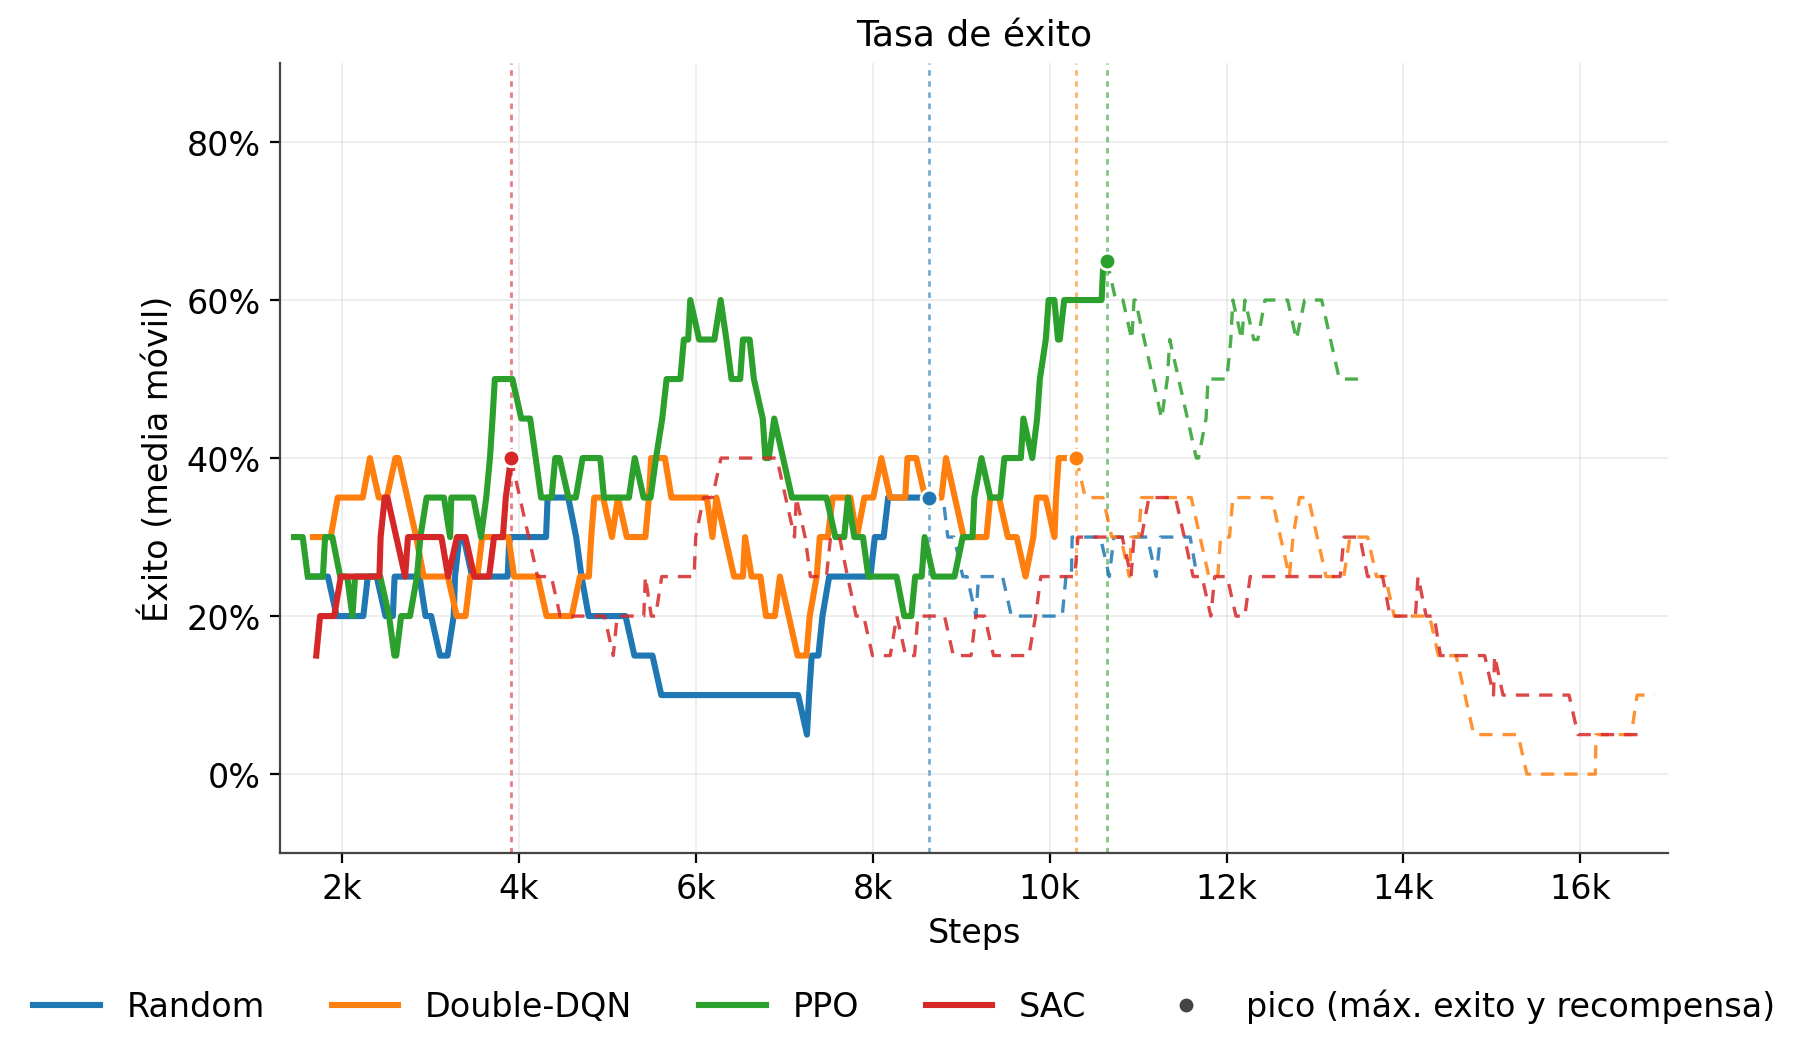
\includegraphics[width=1\textwidth]{imaxes/08_rl/comparativa_rl_exito.png}
  }
  \caption[Tasa de éxito (media móvil, ventana 20)]{Tasa de éxito durante el
  entrenamiento (media móvil, ventana de \num{20} episodios). PPO obtiene el mejor rendimiento,
  seguido de DQN y SAC; los tres superan al agente aleatorio. La línea continua llega hasta
  el mejor \textit{checkpoint} y la discontinua hasta el final del entrenamiento.}
  \label{fig:rl-comparativa-exito}
\end{figure}

\begin{figure}[htbp]
  \centering
  \resizebox{\textwidth}{!}{%
  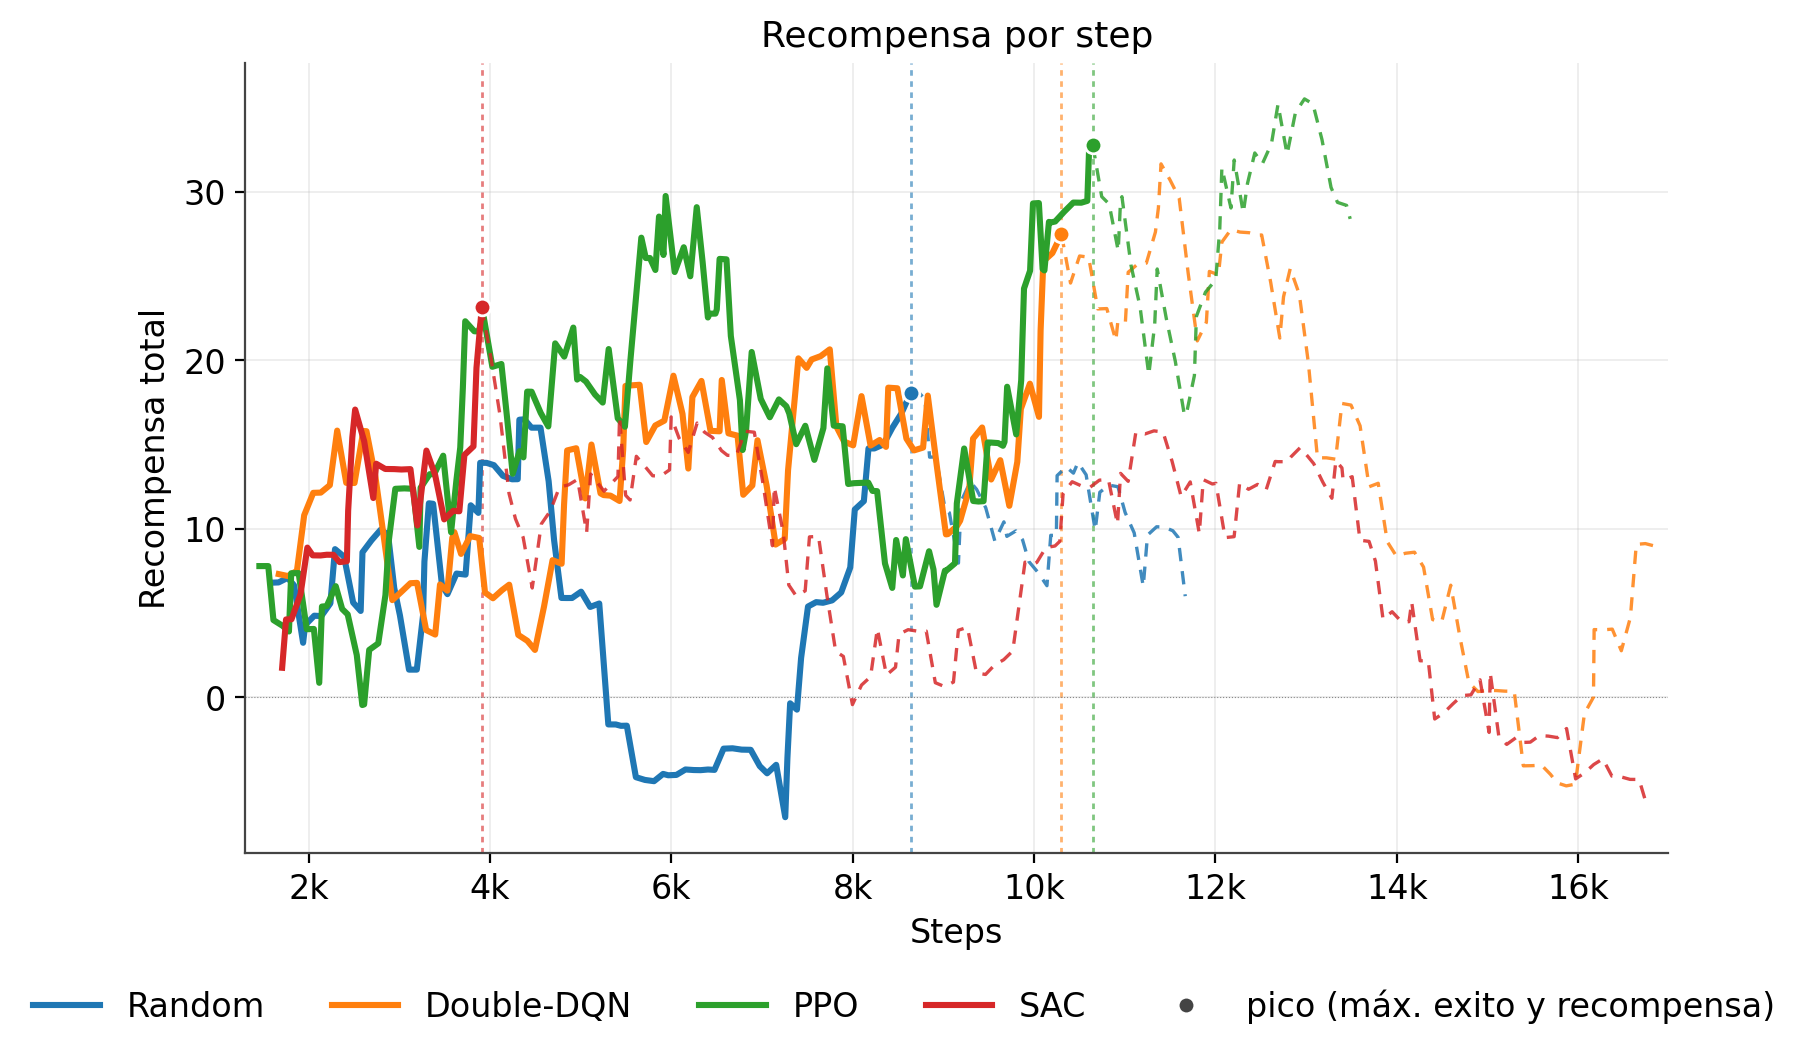
\includegraphics[width=1\textwidth]{imaxes/08_rl/comparativa_rl_recompensa.png}
  }
  \caption[Recompensa por episodio (media móvil, ventana 20)]{Recompensa total por
  episodio durante el entrenamiento (media móvil, ventana de \num{20} episodios). El orden
  coincide con el de la tasa de éxito. La caída final de SAC por debajo de cero es
  coherente con su inestabilidad (Figura~\ref{fig:rl-estabilidad}, página~\pageref{fig:rl-estabilidad}).}
  \label{fig:rl-comparativa-recompensa}
\end{figure}

El algoritmo con mejor rendimiento es \gls{ppo}, alcanza la mayor tasa de éxito en el
pico (\qty{65}{\percent}) y la mayor recompensa (\num{32.75}), y su curva mantiene una tendencia
ascendente, lo que sugiere que con más episodios
podría seguir mejorando. \gls{dqn} y \gls{sac} quedan por detrás, ambos rondando el \qty{40}{\percent}
de éxito en el pico; su tendencia indica un deterioro, aunque para confirmarlo sería necesario
un mayor número de episodios para observar realmente si se estabilizan o siguen cayendo.
Aun así, los tres algoritmos superan a la \gls{baseline} aleatoria (\qty{35}{\percent}, \num{18.04} de
recompensa), lo que confirma que sí hay aprendizaje.

Conviene matizar que las caídas observadas no son principalmente un
problema de exploración, sino la dificultad de la tarea combinada con el
diseño del mundo ya que el punto de aparición se mantiene fijo durante \num{10} episodios
(Sección~\ref{sec:rl-config}, página~\pageref{sec:rl-config}). Si en ese punto no hay árboles cercanos, el agente cae en
un agujero o queda atrapado, encadena varios episodios sin éxito que hunden la media móvil,
independientemente de si el agente aprendió a evitar esas situaciones o no. 
Esto explica por qué la curva final (línea discontinua) no se estabiliza o continúa descendiendo, y refuerza 
la elección del pico de la media móvil frente al \textit{\gls{checkpoint}} final.


\subsection{Estabilidad del entrenamiento}
\label{sec:rl-estabilidad}
La diferencia entre PPO y los otros dos algoritmos no solo está en la tasa de éxito, sino
en la estabilidad del proceso. La Figura~\ref{fig:rl-estabilidad} (página~\pageref{fig:rl-estabilidad}) muestra dos
señales propias de los algoritmos que pueden ayudar a explicar el deterioro de \gls{dqn} y \gls{sac}.

\begin{figure}[htbp]
  \centering
  \resizebox{\textwidth}{!}{%
  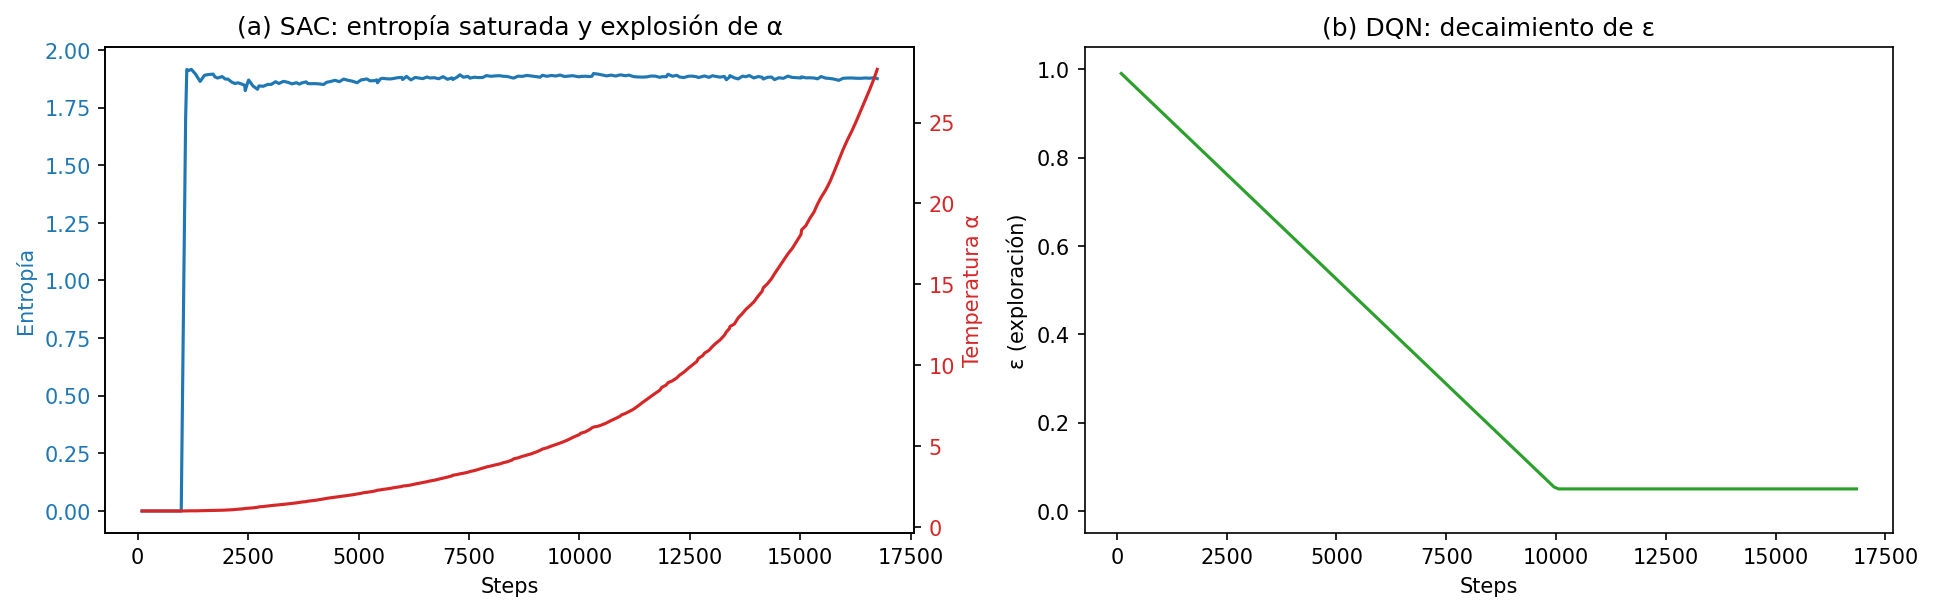
\includegraphics[width=1\textwidth]{imaxes/08_rl/estabilidad_rl.png}
  }
  \caption[Señales de estabilidad de SAC y DQN]{Señales internas del entrenamiento.
  \textbf{(a)}: en SAC, la temperatura $\alpha$ (rojo) se dispara mientras la entropía
  de la \gls{política} (azul) permanece cerca de su máximo, indicando que el término de
  entropía domina y la \gls{política} nunca se vuelve decisiva. \textbf{(b)}: en DQN, el
  decaimiento programado de $\varepsilon$ funciona correctamente. Pero la red
  podría aprovecharse de un mayor periodo de exploración.}
  \label{fig:rl-estabilidad}
\end{figure}

En \gls{sac} (a), la temperatura de entrenamiento ($\alpha$) se ajusta de forma
automática (Sección~\ref{sec:rl-sac}, página~\pageref{sec:rl-sac}). 
En la práctica $\alpha$ no se estabiliza, sino que
crece sin control (de $\sim\num{1}$ a $\sim\num{28}$ al final del entrenamiento), de forma que
la entropía termina dominando a la recompensa, y el agente no llega a fijar
una \gls{política} concreta. Su entropía acaba llegando a $\approx\num{2}$ rápidamente,
indicando que la \gls{política} es casi uniforme y el agente actúa de forma aleatoria.
Esto corresponde con la caída de su recompensa por debajo de cero
(Figura~\ref{fig:rl-comparativa-recompensa}, página~\pageref{fig:rl-comparativa-recompensa}) y
su distribución de acciones (Figura~\ref{fig:rl-acciones}, página~\pageref{fig:rl-acciones}).
Se probaron distintos valores de entropía objetivo (\num{-1}, \num{-2} y \num{-3}), pero en todos 
los casos $\alpha$ continúa creciendo sin control y la \gls{política} no se vuelve decisiva.
No se descarta el rendimiento de SAC, pero su aplicabilidad requiere 
un ajuste más fino de hiperparámetros y un mayor número de episodios de entrenamiento.


En \gls{dqn} (b) la exploración la controla $\varepsilon$, que decae de forma
uniforme de \num{1.0} a \num{0.05} a lo largo de los primeros $\sim\num{10000}$ pasos. 
El mejor rendimiento obtenido por la \gls{dqn} se obtiene alrededor de los $\sim\num{10000}$ pasos.
El punto donde la red comienza su explotación es visible en la Figura~\ref{fig:rl-comparativa-exito} (página~\pageref{fig:rl-comparativa-exito}).
Con un mayor periodo de exploración, la \gls{dqn} podría haber alcanzado un mejor rendimiento 
al poder aprender mejor las variaciones del entorno.


\subsection{Distribución de acciones}
\label{sec:rl-acciones}
La Figura~\ref{fig:rl-acciones} (página~\pageref{fig:rl-acciones}) muestra la distribución de cada una de las siete
acciones durante la evaluación de los cuatro agentes.

El agente \textbf{aleatorio} reparte las acciones de forma uniforme. 
\gls{sac} es muy similar a la versión aleatoria, lo que confirma
el análisis de la sección anterior: la explosión de $\alpha$ lo deja en una \gls{política}
casi aleatoria. \gls{dqn} sí muestra una distribución de aprendizaje; gran parte de las acciones
realizadas son \textit{camera\_down}, seguido de \textit{camera\_up}. Esto corresponde con el proceso de tala
que podría realizar un jugador humano; al talar el tronco que tiene a la altura de los ojos, la red aprende a talar
los troncos adyacentes en el eje vertical. 
\gls{ppo}, en cambio, es el único que reparte el peso entre
las acciones más relevantes de la tarea: \textit{attack}, \textit{move\_forward\_sprint}
y \textit{move\_forward\_jump}, que es justo la combinación de
avanzar hacia un árbol y golpearlo que sigue el experto.

\begin{figure}[htbp]
  \centering
  \resizebox{0.9\textwidth}{!}{%
  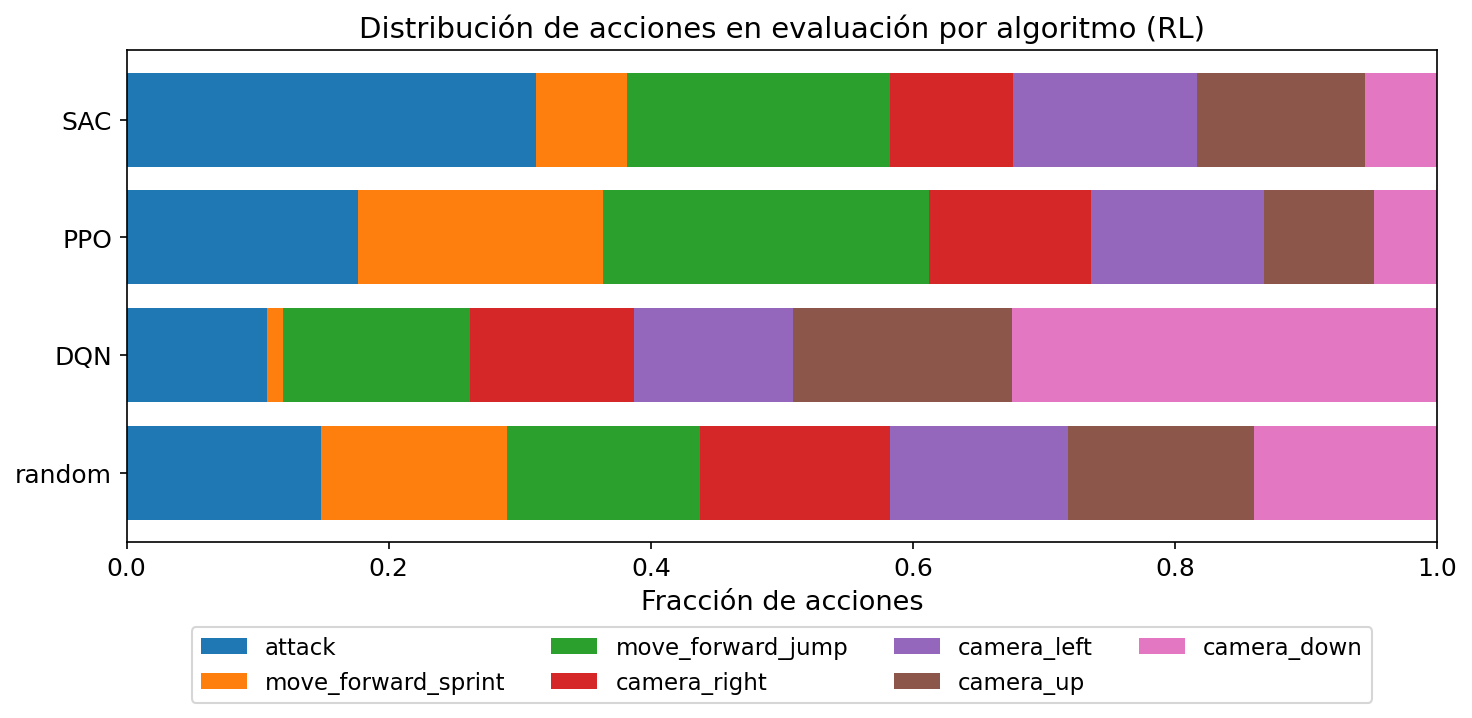
\includegraphics[width=0.8\textwidth]{imaxes/08_rl/accion_dist_rl.png}
   }
  \caption[Distribución de acciones por algoritmo de refuerzo]{Fracción de cada acción durante la
  evaluación. SAC y el agente aleatorio reparten las acciones de forma casi uniforme; DQN
  se concentra en \textit{camera\_down}; PPO favorece las acciones
  productivas de la tarea (\textit{attack} y movimiento).}
  \label{fig:rl-acciones}
\end{figure}

\begin{figure}[htbp]
  \centering
  \resizebox{0.8\textwidth}{!}{%
  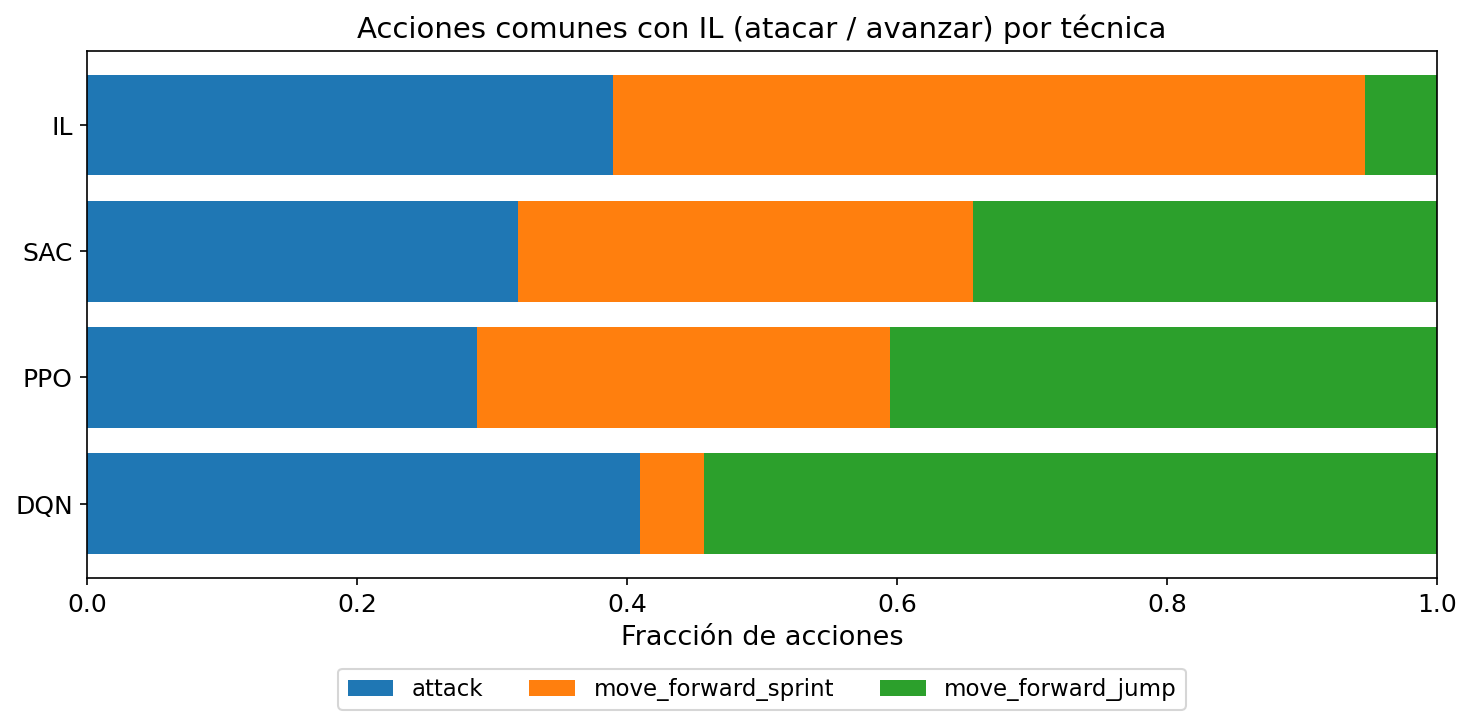
\includegraphics[width=0.8\textwidth]{imaxes/08_rl/accion_dist_comun.png}
  }
  \caption[Distribución de acciones por algoritmo de refuerzo con el mismo espacio de acciones que el agente de imitación.]{
  Fracción de cada acción durante la
  evaluación, eliminando las acciones que no están en el espacio de acciones del agente de imitación.}
  \label{fig:rl-acciones-comun}
\end{figure}

Además, la Figura~\ref{fig:rl-acciones-comun} (página~\pageref{fig:rl-acciones-comun}) 
muestra la distribución de acciones de los tres algoritmos de refuerzo, eliminando las acciones que no están en el espacio
de acciones de imitación (Sección~\ref{sec:il-arch-dual}, página~\pageref{sec:il-arch-dual}). Es decir, eliminando el componente
de la cámara, para ver si los algoritmos de refuerzo aprenden el mismo tipo de distribución que
la imitación del experto. El más cercano a la distribución es curiosamente el \textbf{DQN}, 
que aunque presenta un éxito menor al de PPO, sí aprende a moverse hacia el árbol y golpearlo.
Aunque con las acciones de movimiento intercambiadas en relación al \gls{il}, el 
\textit{move\_forward\_sprint} en \gls{dqn} tiene la misma distribución que
\textit{move\_forward\_jump} en \gls{il}, y viceversa.  

\subsection{Discusión}
El refuerzo parece ser la técnica con un mayor horizonte de desarrollo, pero en consecuencia
presenta el mayor coste computacional y temporal. La literatura (Capítulo~\ref{chap:sota}) 
muestra que el refuerzo puede aprender tareas de \textit{Minecraft} como la tala de árboles,
o la obtención de diamante~\cite{guss2019minerl}. Pero a coste de un inmenso conjunto de datos y tiempo de entrenamiento.
El número de episodios de entrenamiento utilizados en este trabajo es muy bajo en comparación con
otros trabajos. Por ejemplo, los agentes de \textit{MineRL}~\cite{guss2019minerl} emplean para la misma tarea 
de tala unos \num{1500} episodios (del orden de \num{12} millones de pasos), lo que en nuestro entorno equivaldría a unas
\num{1800} horas de cómputo (unos \num{75} días continuos) por algoritmo.

Los resultados de esta iteración muestran que el refuerzo es capaz de aprender la tarea, aunque
sin llegar a un rendimiento comparable al de la aproximación simbólica o de imitación. Pero también muestran 
que el refuerzo puede no requerir de un conjunto de datos y
tiempo de cómputo tan grande como el de \textit{MineRL}~\cite{guss2019minerl}. Con un conjunto de datos de 
\num{200} episodios (unas \num{2} horas de cómputo) es posible obtener un rendimiento aceptable
que muestre tendencias hacia un rendimiento óptimo.